\documentclass{article}
\usepackage{graphicx} % Required for inserting images
\usepackage{pgfplots}
\usepackage{adjustbox}
\usepackage{multicol}
\usepackage{float}
\usepackage{booktabs}
\usepackage[a4paper, margin=1in]{geometry} % Adjust margins as needed
\usepackage{mathptmx} % Times New Roman-like font
\usepackage{hyperref} % For hyperlinks and references
\usepackage{listings}
\usepackage{amsmath}

% Define a highlight color
\hypersetup{
    colorlinks=true,
    linkcolor=blue,
    citecolor=yellow,
    urlcolor=yellow
}
\title{ACML Report}
\author{
Sayfullah Jumoorty (2430888)
\\\\
Pratham Tejas Berawala (2441515)
\\ \\
Muhammed Muaaz Dawood (2425639)
\\ \\
Mujammil Mohsin Gulam Sakhidas (2436109)
}
\date{May 2024}

\begin{document}

\maketitle

\section{Dataset}
\subsection{Data Source} \label{SnD}
We utilized the CIFAR-10 dataset for this project. CIFAR-10 is an established computer-vision dataset used for object recognition tasks. Instead of downloading the full dataset from Kaggle, we imported it directly in our code using Keras and TensorFlow, leveraging it for ease of use and integration. The Python Keras dataset is a subset of the 80 million tiny images from Kaggle and consists of 60,000 32x32 color images, each belonging to one of 10 object classes: airplane, automobile, bird, cat, deer, dog, frog, horse, ship, and truck. Each class contains 6,000 images.
The dataset was collected by Alex Krizhevsky, Vinod Nair, and Geoffrey Hinton and has been widely used in the machine learning community for benchmarking algorithms.

% The dataset is divided into 50,000 training images and 10,000 testing images. Each image is a 32x32 pixel RGB image with pixel values ranging from 0 to 255. The labels are provided as integers corresponding to the 10 object classes.
% By utilizing this dataset, we aim to explore and implement various machine learning techniques for image classification and improve the accuracy and efficiency of these models.
\subsection{Objectives}
The primary objective of utilizing the CIFAR-10 dataset in this project is to develop, train, and evaluate a machine learning model capable of accurately classifying images into one of the 10 predefined object categories: airplane, automobile, bird, cat, deer, dog, frog, horse, ship, and truck. 
\\\\
Specific objectives include:
\begin{itemize}
    \item Preprocessing the dataset to ensure it is in an optimal format for model training.
    \item Designing and implementing a convolutional neural network (CNN) to effectively learn from the CIFAR-10 images and generalize to unseen data.
    \item Training the model using the training dataset and fine-tuning hyperparameters to achieve the best performance.
    \item Evaluating the model’s performance on the test dataset using metrics such as accuracy, precision, recall, and F1-score.
\end{itemize}


\section{Dataset Pre-Processing}
 
In our implementation, the dataset preprocessing includes the following steps:

\begin{enumerate}

    \item \textbf{Loading the Dataset:} 

    The CIFAR-10 dataset consists of 60,000 $32 \times 32$ color images, with the dataset already split into 50,000 training images and 10,000 testing images. After loading and preprocessing this data, scikit-learn's \texttt{train\_test\_split} function is used to further split the 50,000 training images into a training set $(x_{\text{train}}, y_{\text{train}})$ comprising 80\% of the data, and a validation set $(x_{\text{val}}, y_{\text{val}})$ comprising the remaining 20\%, with a fixed \texttt{random\_state} for reproducibility. The original 10,000 test images $(x_{\text{test}}, y_{\text{test}})$ remain as the test set. During model training, the validation set is used for hyperparameter tuning and model selection, while the test set evaluates the final trained model's performance.


    \item \textbf{Normalization:} To ensure the pixel values are on a comparable scale, we normalize the image data by scaling the pixel values to the range [0, 1]. This is done by dividing each pixel value by 255.0.

    \item \textbf{One-Hot Encoding:} The class labels provided in the dataset are integers ranging from 0 to 9. For training the neural network, we convert these labels to one-hot encoded vectors using TensorFlow's \textbf{Categorical} function which converts a class vector (integers) into a binary class matrix.

    \item \textbf{Data Augmentation:} To improve the generalization of the model and prevent over-fitting, we apply data augmentation techniques to the training images. This includes:
    \begin{itemize}
        \item \textbf{Rotation:} Randomly rotating the images within a range of 15 degrees.
        \item \textbf{Width Shift:} Randomly shifting the images horizontally by 10% of the total width.
        \item \textbf{Height Shift:} Randomly shifting the images vertically by 10% of the total height.
        \item \textbf{Horizontal Flip:} Randomly flipping the images horizontally.
    \end{itemize}
    Data augmentation is implemented using TensorFlow's \textbf{ImageDataGenerator} class, which generates batches of tensor image data with real-time data augmentation.

\end{enumerate}
By performing these preprocessing steps, we ensure that the data fed into the neural network model is in an optimal format, which helps improve the accuracy and robustness of the model.


\section{The Model}

In this section, we describe the choice and implementation of the model used for image classification on the CIFAR-10 dataset.

\subsection{Model Choice: Convolutional Neural Network (CNN)}

The model chosen for this implementation is a Convolutional Neural Network (CNN). CNNs are particularly well-suited for image classification tasks due to their ability to capture spatial hierarchies in images. The specific architecture of the CNN we developed in this implementation is designed to handle the CIFAR-10 dataset, which consists of 60,000 32x32 color images in 10 classes, with 6,000 images per class.

\subsection{Machine Learning Algorithm: Supervised Learning}

The learning algorithm employed is supervised learning, specifically using the categorical cross-entropy loss function. This is appropriate for classification tasks where the model is trained to predict the probability distribution over multiple classes.

\subsection{Model Iterations}

To find a suitable model and fine-tune it for the CIFAR-10 dataset, several experiments were conducted with different architectures and hyperparameters. The goal was to improve the model's performance and generalization ability. The following experiments were performed:

\begin{enumerate}
    \item \textbf{Baseline Model:}
    \begin{itemize}
        \item A simple CNN architecture was used as a starting point, consisting of one convolutional layer, max pooling, and dense layers.
        \item This model achieved a test accuracy of 0.6065, serving as a baseline for further improvements.
     %  2 images side by side
    \begin{figure}[H]
        \centering
        \begin{minipage}{0.45\textwidth}
            \centering
            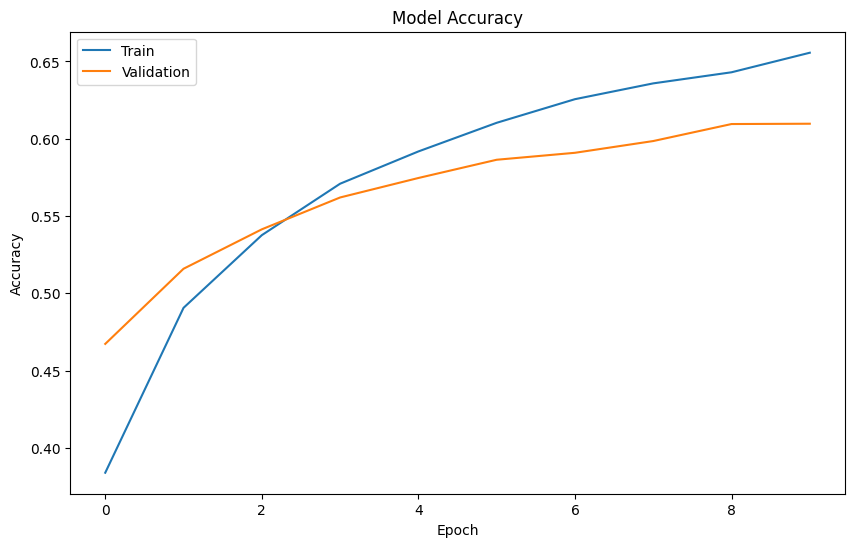
\includegraphics[width=\textwidth]{BaselineMA.png}
            \caption{Baseline Model Accuracy}
            \label{BMA}
        \end{minipage}
        \hfill
        \begin{minipage}{0.45\textwidth}
            \centering
            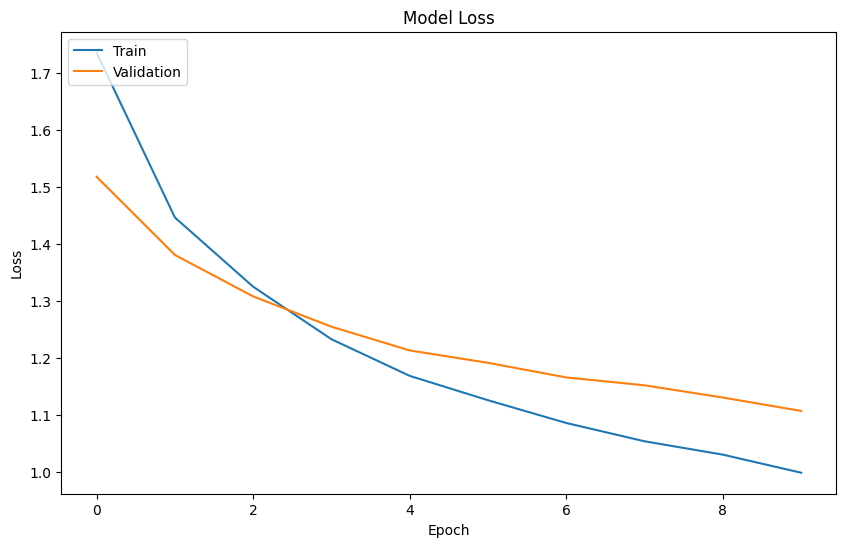
\includegraphics[width=\textwidth]{BaselineML.png}
            \caption{Baseline Model Loss}
            \label{BML}
        \end{minipage}
    \end{figure}
        
    \end{itemize}
    
    \item \textbf{Increasing Model Depth:}
    \begin{itemize}
        \item The model architecture was deepened by adding more convolutional layers.
        \item The final architecture consisted of three sets of two convolutional layers, each followed by max pooling.
        \item Increasing the depth allowed the model to learn more complex features, resulting in an improved test accuracy of 0.7137.

        \begin{figure}[H]
        \centering
        \begin{minipage}{0.45\textwidth}
            \centering
            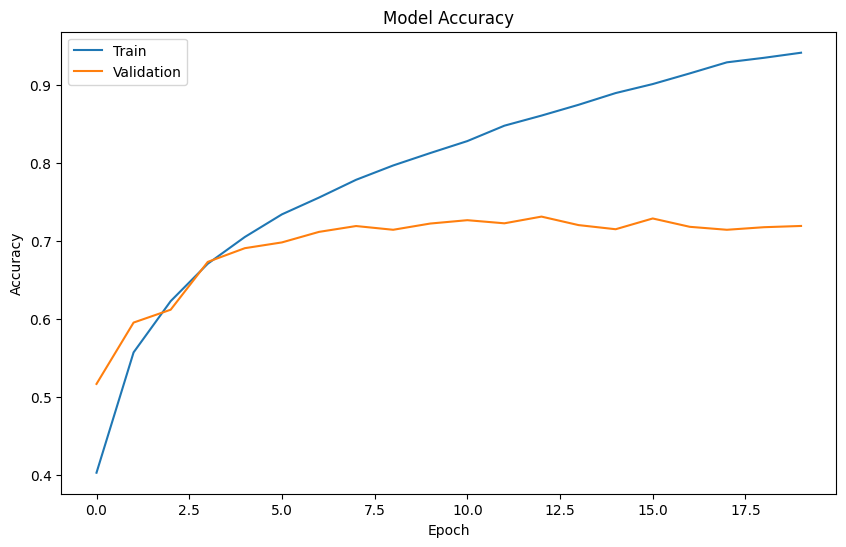
\includegraphics[width=\textwidth]{DepthMA.png}
            \caption{Depth  Model Accuracy}
            \label{DMA}
        \end{minipage}
        \hfill
        \begin{minipage}{0.45\textwidth}
            \centering
            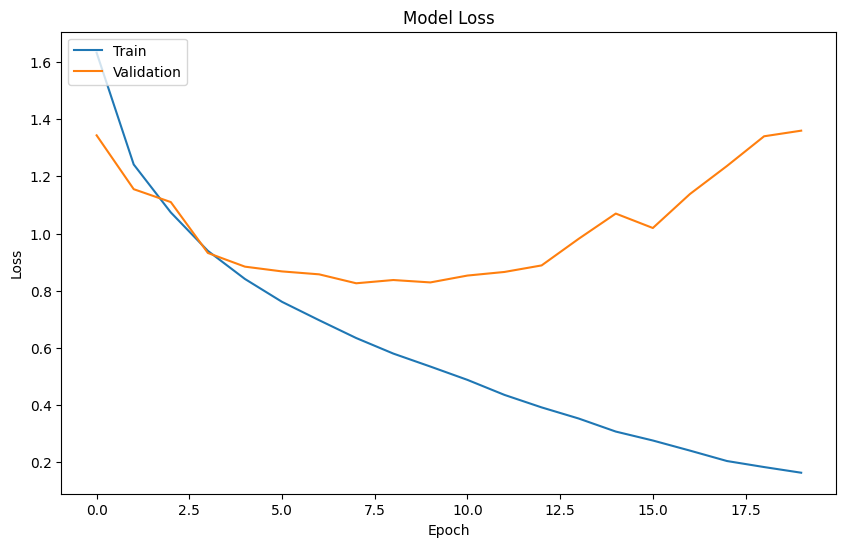
\includegraphics[width=\textwidth]{DepthML.png}
            \caption{Depth Model Loss}
            \label{DML}
        \end{minipage}
    \end{figure}
        
    \end{itemize}
    
   
    
    \item \textbf{Batch Normalization:}
    \begin{itemize}
        \item Batch normalization layers were added after each convolutional layer.
        \item Batch normalization helps stabilize the training process by normalizing the activations and reducing internal covariate shift.
        \item The model achieved a higher training accuracy of 0.9858, but the test accuracy was 0.7227 suggesting potential over-fitting however it still gave a better accuracy than the previous model.
        
    \end{itemize}
    
    \begin{figure}[H]
        \centering
        \begin{minipage}{0.45\textwidth}
            \centering
            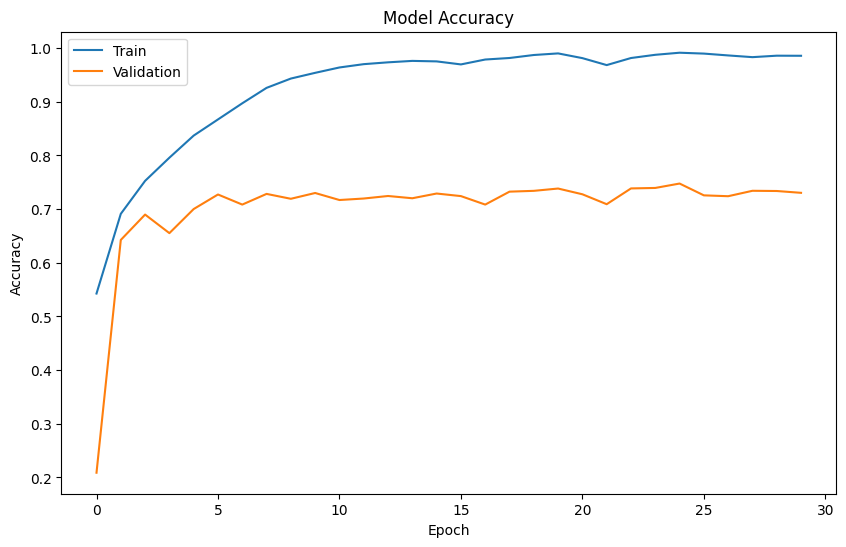
\includegraphics[width=\textwidth]{BatchMA.png}
            \caption{Batch Normalization  Model Accuracy}
            \label{BNMA}
        \end{minipage}
        \hfill
        \begin{minipage}{0.45\textwidth}
            \centering
            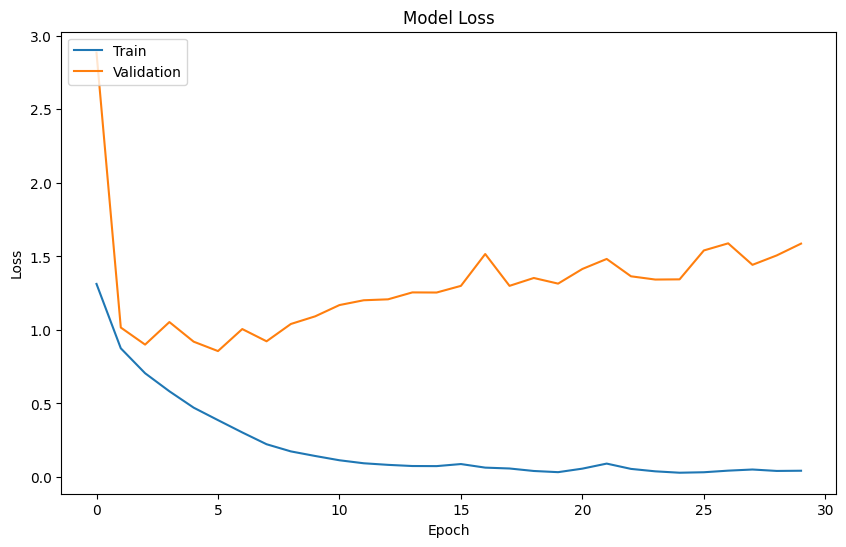
\includegraphics[width=\textwidth]{BatchML.png}
            \caption{Batch Normalization Model Loss}
            \label{BNML}
        \end{minipage}
    \end{figure}
    
    \item \textbf{Data Augmentation:}
    \begin{itemize}
        \item Image data augmentation techniques were applied to expand the training dataset and improve the model's ability to generalize.
        \item Techniques such as rotation, width and height shifts, and horizontal flipping were used.
        \item Data augmentation helped the model learn invariance to these transformations, resulting in an improved test accuracy of 0.7593.
    \end{itemize}

    \begin{figure}[H]
        \centering
        \begin{minipage}{0.45\textwidth}
            \centering
            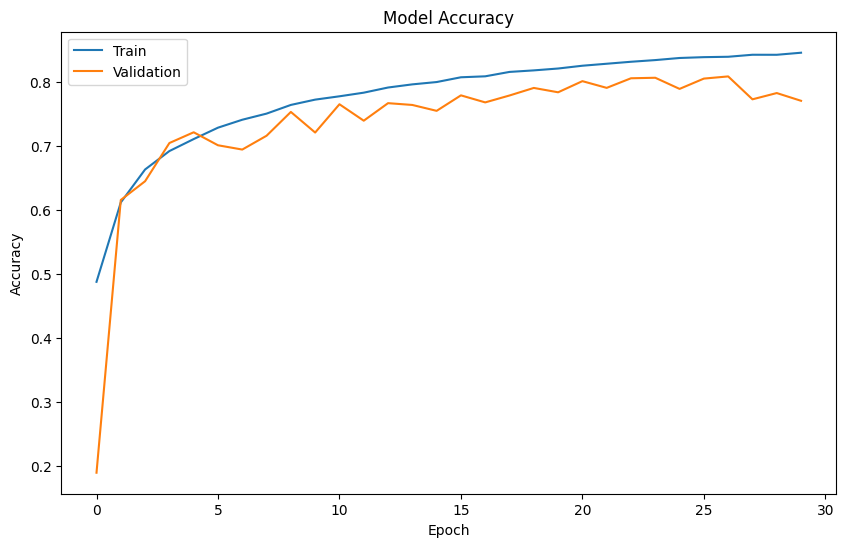
\includegraphics[width=\textwidth]{DataArgMA.png}
            \caption{Data Argumentation  Model Accuracy}
            \label{DAMA}
        \end{minipage}
        \hfill
        \begin{minipage}{0.45\textwidth}
            \centering
            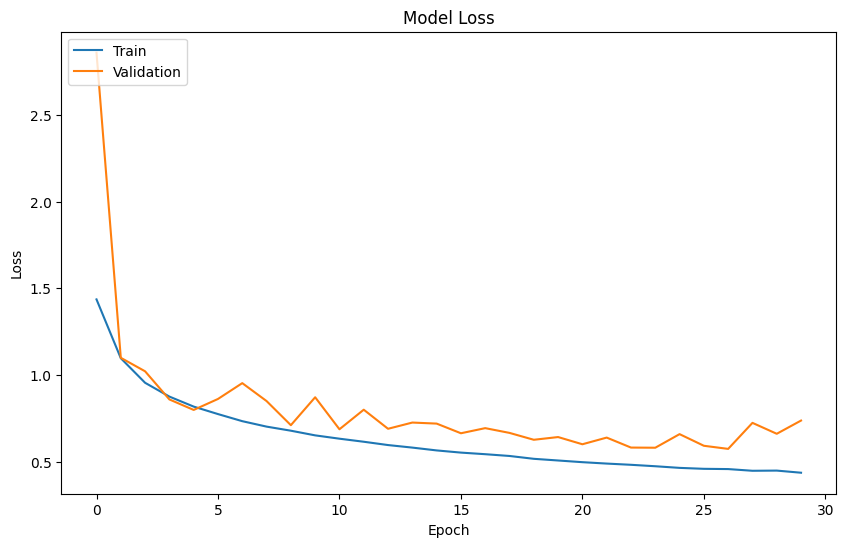
\includegraphics[width=\textwidth]{DataArgML.png}
            \caption{Data Argumentation Model Loss}
            \label{DAML}
        \end{minipage}
    \end{figure}
    
    \item \textbf{Learning Rate and Optimizer:}
    \begin{itemize}
        \item Experiments were conducted with different learning rates (0.001, 0.01, 0.1) and optimizers (Adam, SGD).
        \item The Adam optimizer with a learning rate of 0.01 yielded the best test accuracy of 0.7889.
        \item Our findings are supported by a comparative study on the performance of different optimizers on deep learning tasks using the CIFAR-10 dataset, as seen in \ref{fig:optimizers}. The figure shows that while the Adam optimizer quickly reaches high accuracy, other optimizers like RMSprop, Adadelta, and Adagrad also achieve similar accuracy levels but with varying rates of convergence. In contrast, SGD converges much more slowly and requires more epochs to reach comparable accuracy.
    \end{itemize}

    \begin{figure}[H]
        \centering
        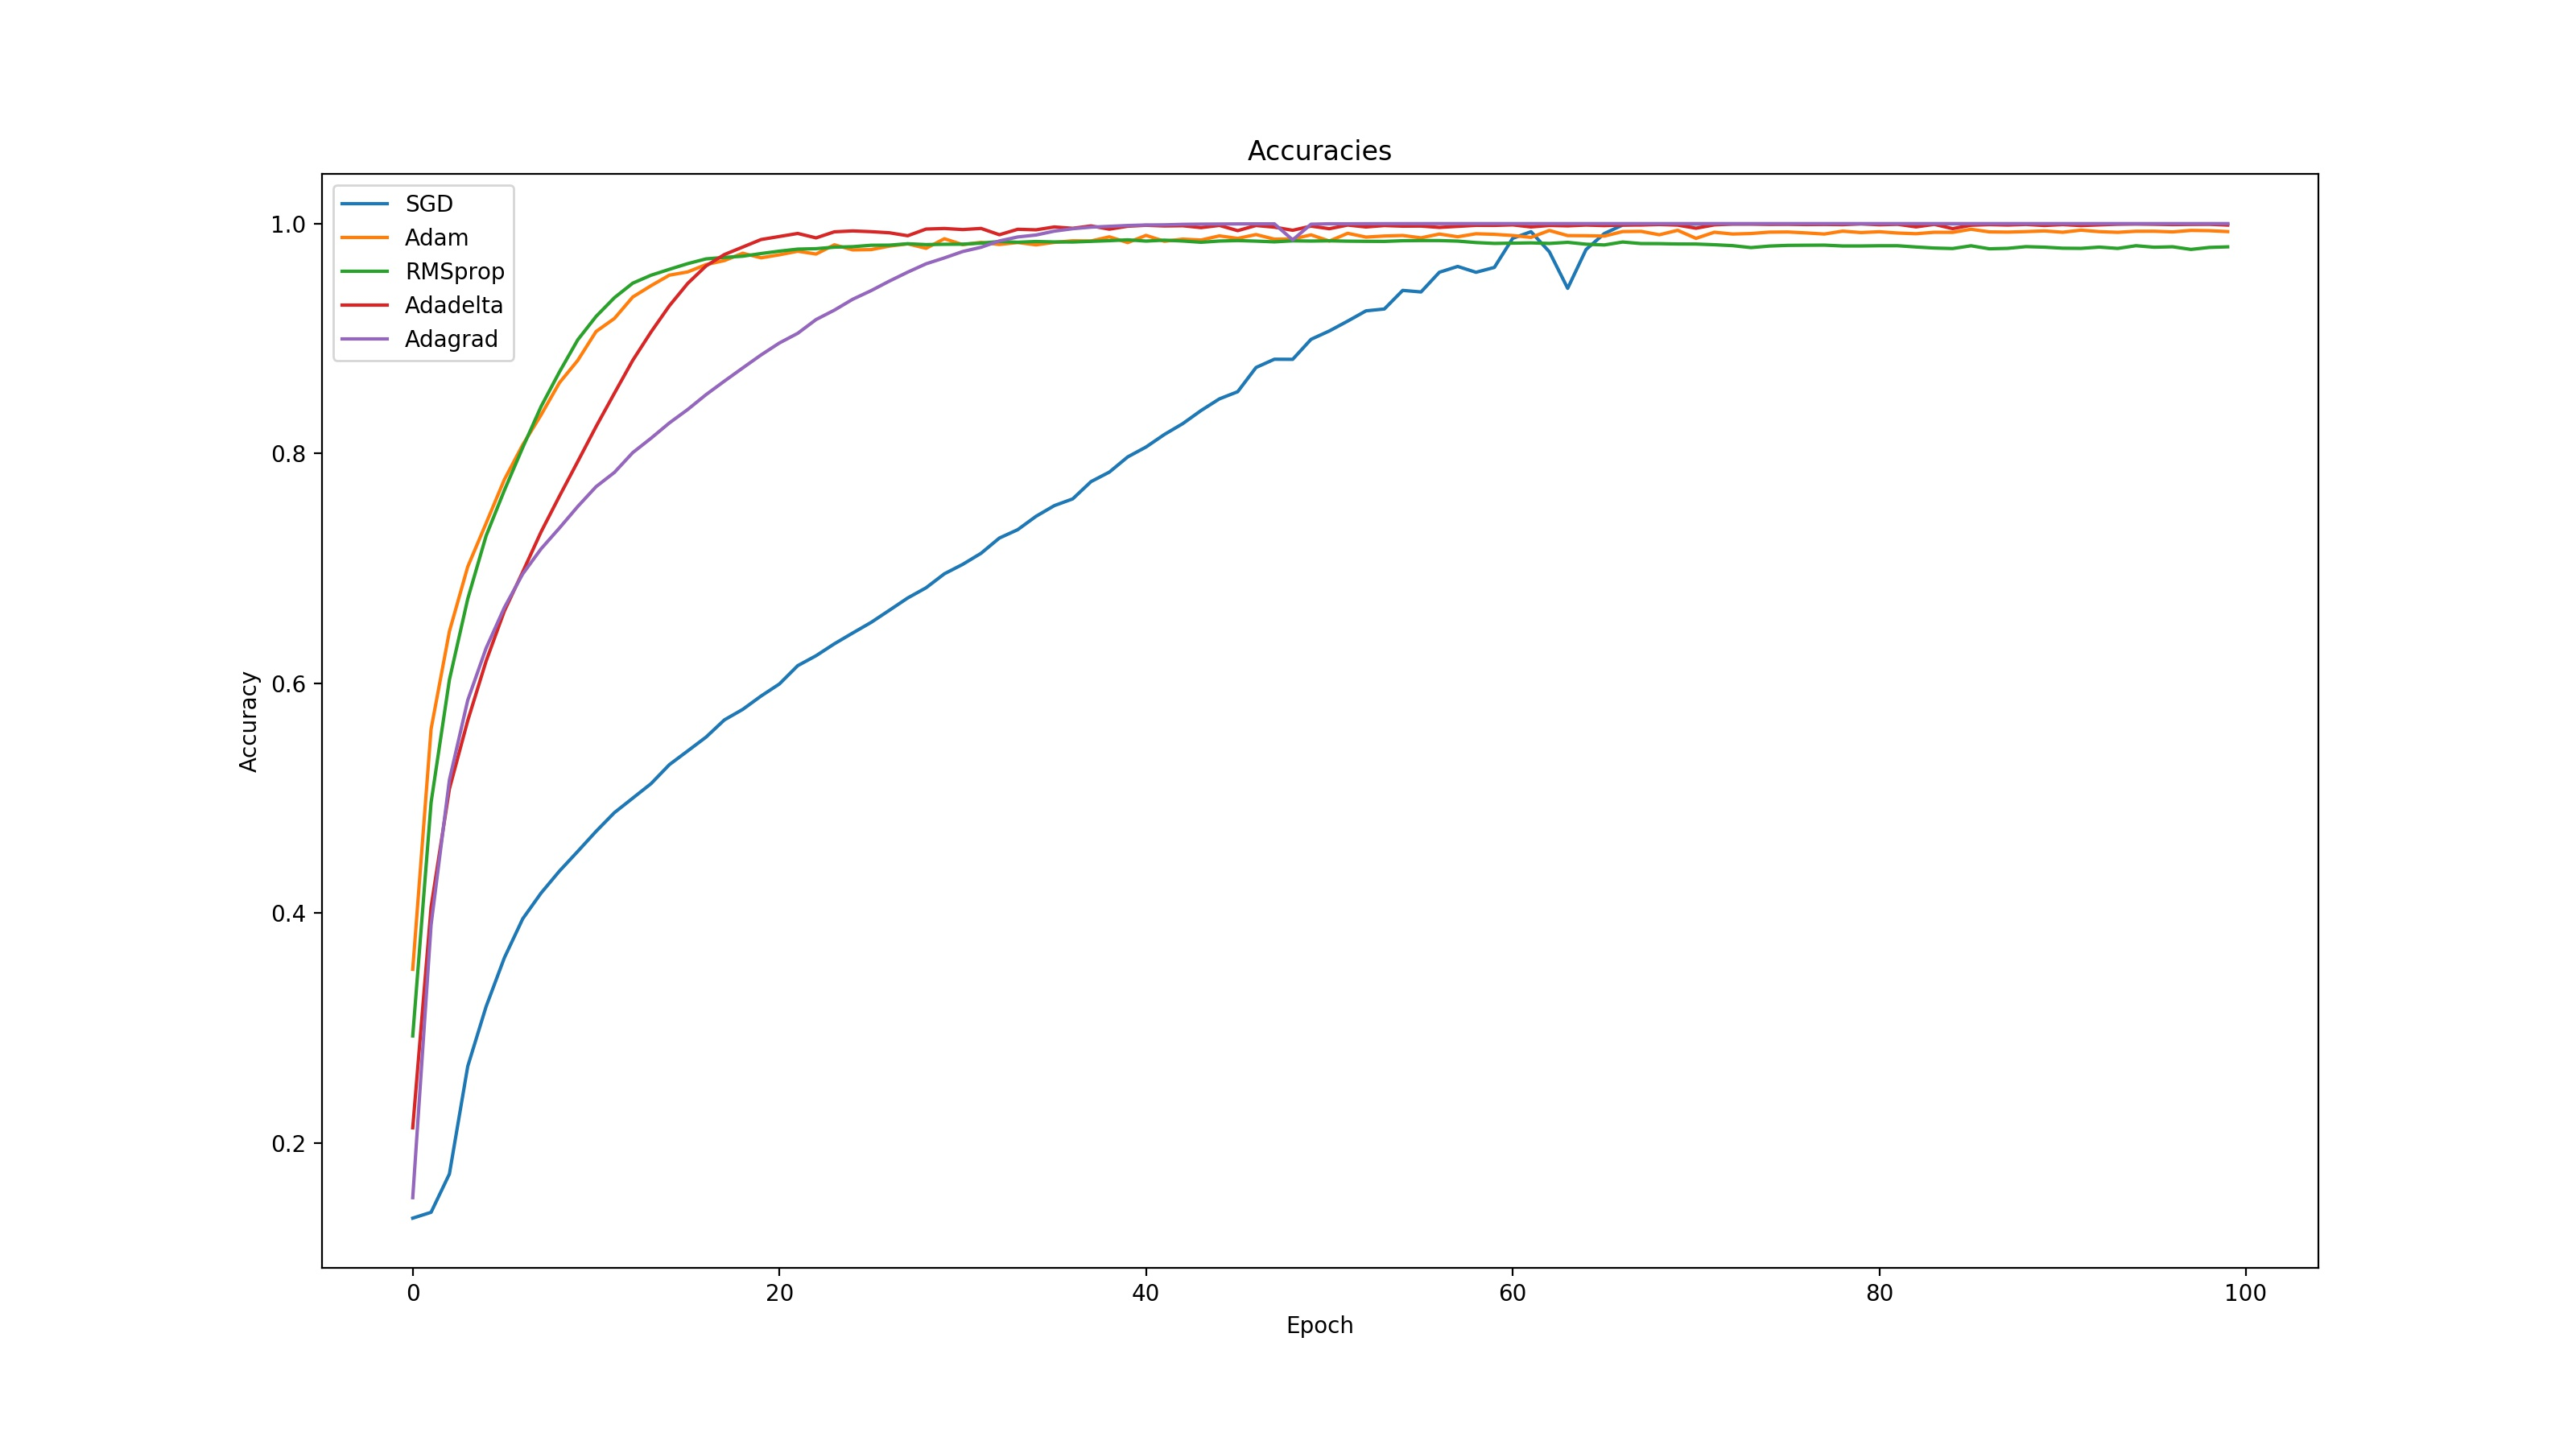
\includegraphics[width=0.9\textwidth]{optimizer-accuracies.jpg}
        \caption{Different Optimizer Results}
        \label{fig:optimizers}
    \end{figure}

    \begin{figure}[H]
        \centering
        \begin{minipage}{0.45\textwidth}
            \centering
            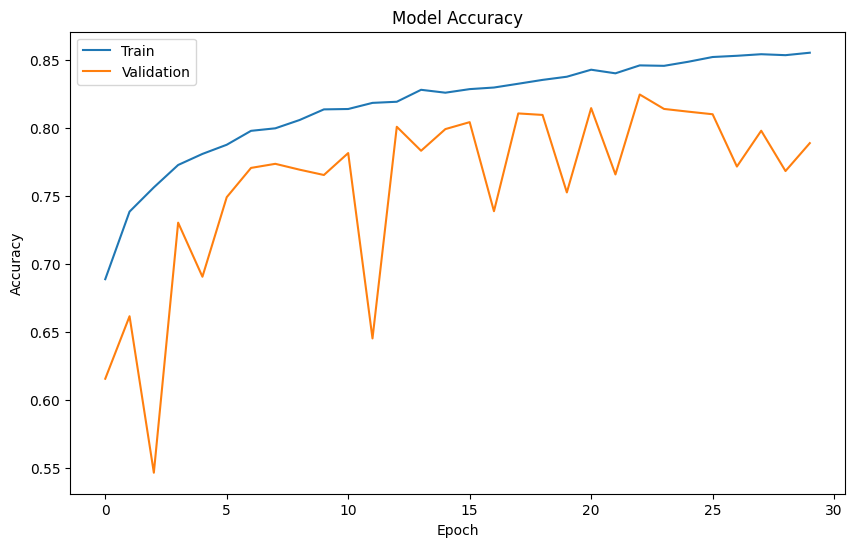
\includegraphics[width=\textwidth]{LRMA.png}
            \caption{Best optimizer Model Accuracy}
            \label{LMA}
        \end{minipage}
        \hfill
        \begin{minipage}{0.45\textwidth}
            \centering
            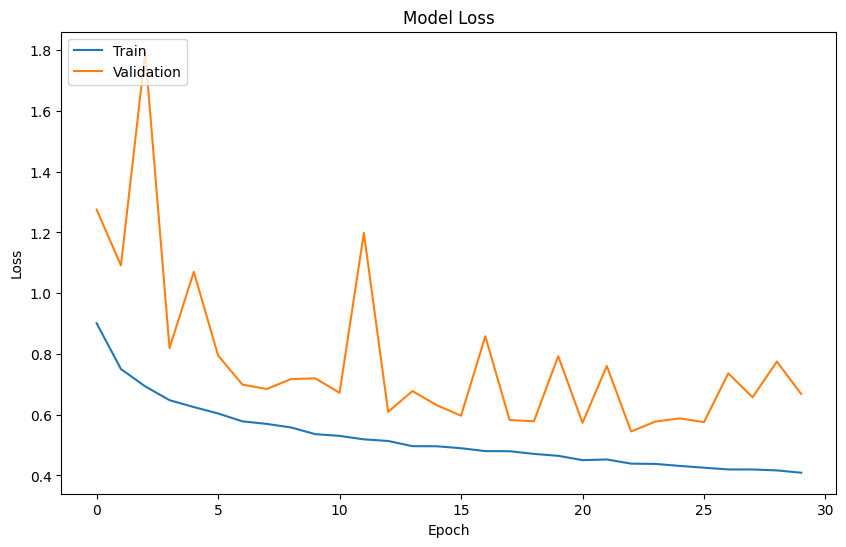
\includegraphics[width=\textwidth]{LRML.png}
            \caption{Best optimizer Model Loss}
            \label{LML}
        \end{minipage}
    \end{figure}
    
    \item \textbf{Early Stopping:}
    \begin{itemize}
        \item Early stopping was implemented to prevent over-fitting and find the optimal number of training epochs.
        \item The model's performance on the validation set was monitored, and training was stopped if the validation loss did not improve for 10 epochs.
        \item Early stopping helped achieve a high test accuracy of 0.8313, demonstrating its effectiveness in preventing over-fitting.
    \end{itemize}


    \begin{figure}[H]
        \centering
        \begin{minipage}{0.45\textwidth}
            \centering
            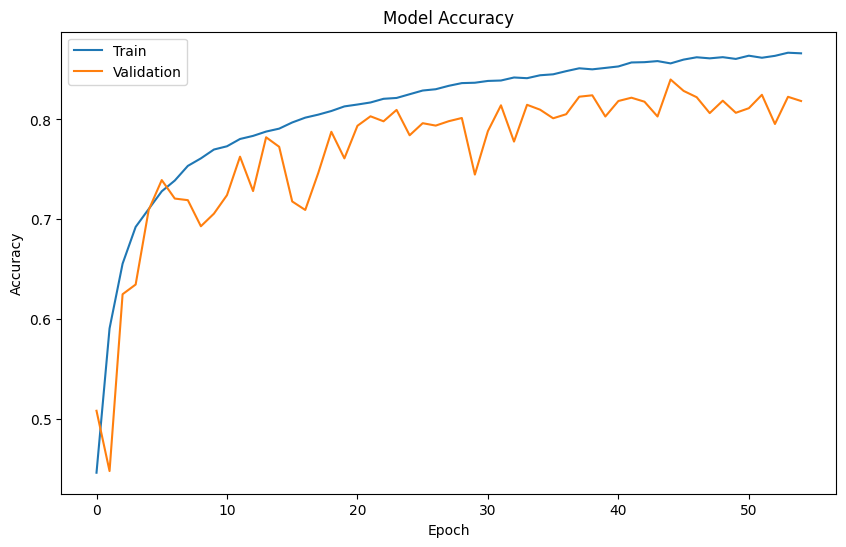
\includegraphics[width=\textwidth]{BestHyperEarlyStoppingMA.png}
            \caption{ Early Stopping Model Accuracy}
            \label{ESMA}
        \end{minipage}
        \hfill
        \begin{minipage}{0.45\textwidth}
            \centering
            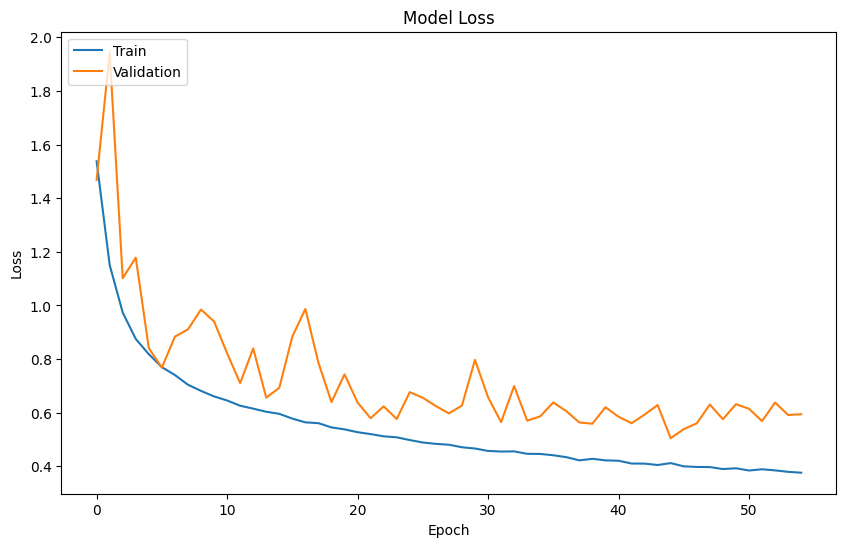
\includegraphics[width=\textwidth]{BestHyperEarlyStoppingML.png}
            \caption{ Early Stopping Model Loss}
            \label{ESML}
        \end{minipage}
    \end{figure}

     \item \textbf{Regularization Techniques:}
    \begin{itemize}
        \item Dropout layers were introduced after each max pooling layer and before the final dense layer.
        \item Dropout helps prevent over-fitting by randomly dropping out a fraction of the neurons during training.
        \item The test accuracy resulted to 0.7811, averaging below 0.8 almost all the time, indicating the ineffectiveness of regularization in reducing over-fitting in this specific case.
    \end{itemize}

        \begin{figure}[H]
        \centering
        \begin{minipage}{0.45\textwidth}
            \centering
            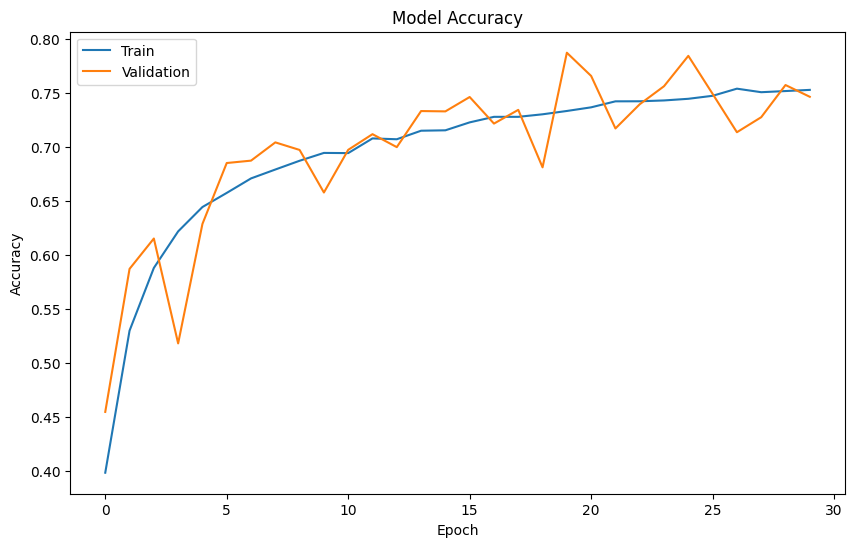
\includegraphics[width=\textwidth]{DropoutMA.png}
            \caption{Dropout Model Accuracy}
            \label{DOMA}
        \end{minipage}
        \hfill
        \begin{minipage}{0.45\textwidth}
            \centering
            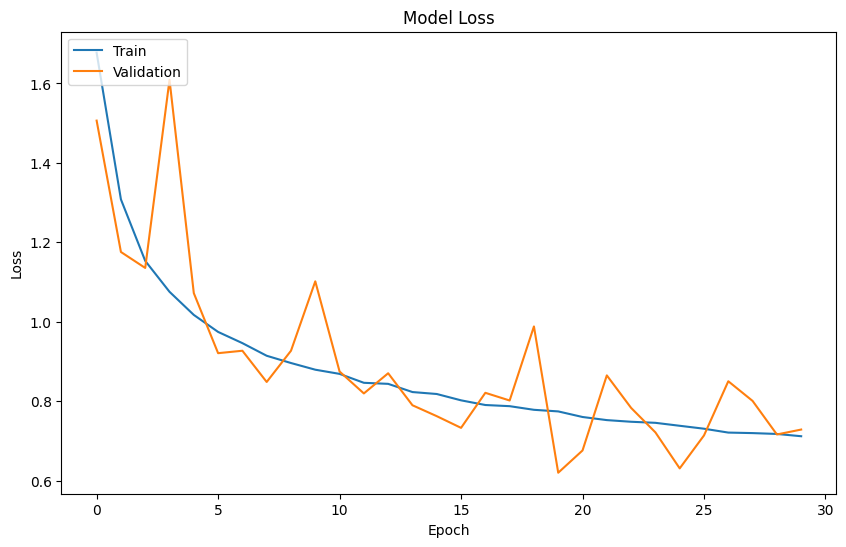
\includegraphics[width=\textwidth]{DropoutML.png}
            \caption{Dropout Model Loss}
            \label{DOML}
        \end{minipage}
    \end{figure}
    
\end{enumerate}

\begin{itemize}
\item The learning rate of 0.01 was selected because it offered a good balance between fast convergence and training stability, allowing the model to learn effectively without causing oscillations or divergence.
\item The Adam optimizer was chosen due to its ability to achieve high accuracy quickly and efficiently. It often leads to better generalization in various deep learning tasks compared to other optimizers.
\item The number of epochs was set to 100 with early stopping to provide ample training time, ensuring the model could learn sufficiently from the data while early stopping helped to mitigate the risk of over-fitting.
\item The batch size of 128 was used as it strikes an optimal balance between computational efficiency and the stability of gradient updates, allowing for effective learning without exhausting memory resources.
\end{itemize}
\vspace{0.5cm}
In conclusion, the experiments conducted helped identify the most suitable model architecture and hyperparameters for the CIFAR-10 dataset. The final model, which incorporated data augmentation, batch normalization, and early stopping, achieved a test accuracy of 0.8313, demonstrating significant improvement over the baseline model. The choice of hyperparameters was guided by empirical results and common practices, leading to a well-performing and generalized model.


\section{Final Model}

The final model developed for image classification on the CIFAR-10 dataset represents a culmination of iterative experimentation and refinement. Through a series of model iterations, encompassing adjustments to architecture, hyperparameters, and various techniques, we aimed to enhance both accuracy and generalization. Our model, a Convolutional Neural Network (CNN) augmented with data augmentation, batch normalization, and early stopping, achieved a notable test accuracy of 0.84, selected from hundreds of runs done on the MSL Cluster.
\\\\
The selection of optimal hyperparameters, informed by empirical evidence and best practices, facilitated robust learning while mitigating the risk of over-fitting. The training accuracy and loss curves for this final model are shown in Figure \ref{fig:finalModelGraphs}, respectively. Similarly, it illustrates the validation accuracy and loss curves, which were used for early stopping to prevent over-fitting.
\\\\
By systematically exploring various configurations and techniques, we successfully identified a model capable of delivering improved performance compared to baseline iterations. This final model stands as a testament to the efficacy of meticulous experimentation in the pursuit of superior machine learning outcomes.

\begin{figure}[H]
\centering
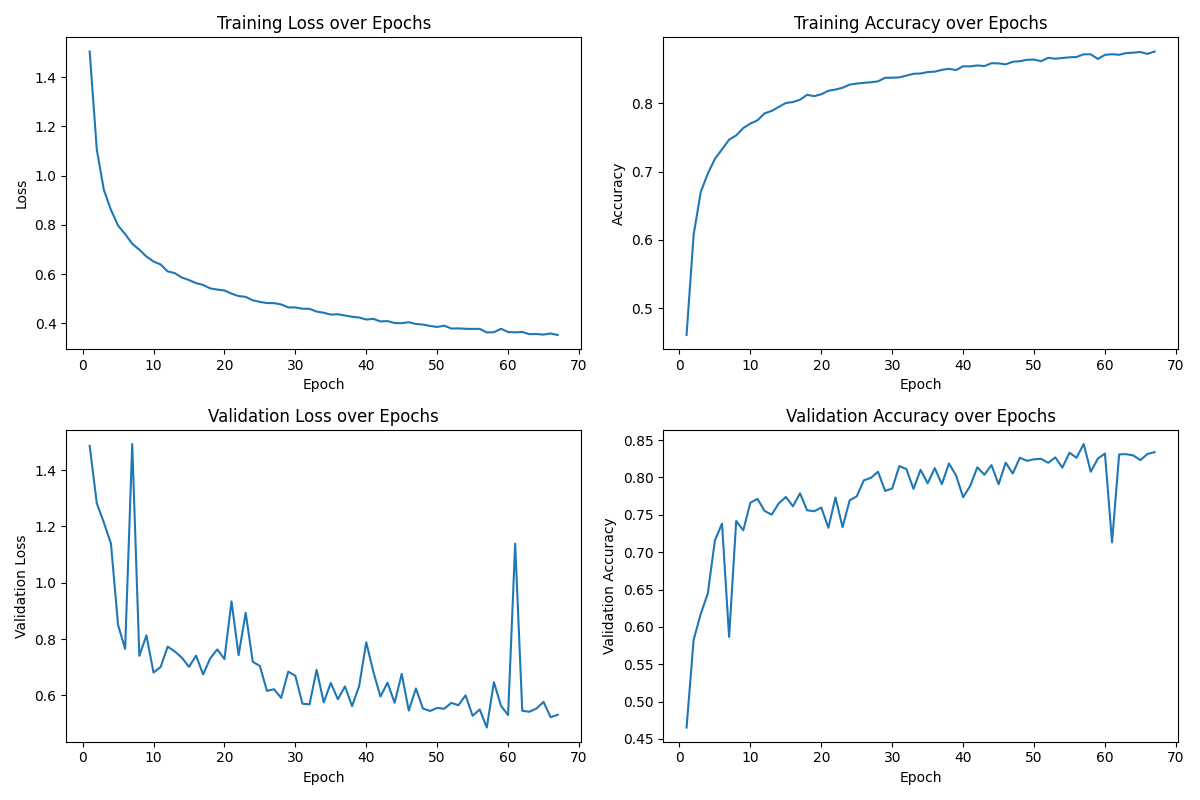
\includegraphics[width=0.8\textwidth]{finalModelGraphs.png}
\caption{Final Model Graphs}
\label{fig:finalModelGraphs}
\end{figure}

\section{Results}

The latest results obtained from running the chosen model on the MSL cluster, show a test accuracy of 0.84. A detailed analysis of the classification report, shown in Figure \ref{fig:class_scores}, reveals promising performance across all classes, with precision, recall, and F1-score metrics consistently above 0.80 for most categories. Particularly noteworthy are the high scores for automobile, ship, and truck classes, indicating robust classification capabilities for transportation-related objects.
\\\\
However, slight discrepancies in precision and recall metrics across classes, as illustrated in Figure \ref{fig:scores_plot}, suggest potential areas for further optimization or fine-tuning. The confusion matrix in Figure \ref{fig:confusion_matrix} provides a visual representation of the model's performance, highlighting the classes with higher misclassification rates.
\\\\
Overall, the heightened test accuracy and balanced performance metrics underscore the efficacy of our final model, affirming its readiness for real-world deployment and validation in diverse scenarios.

\begin{figure}[H]
\centering
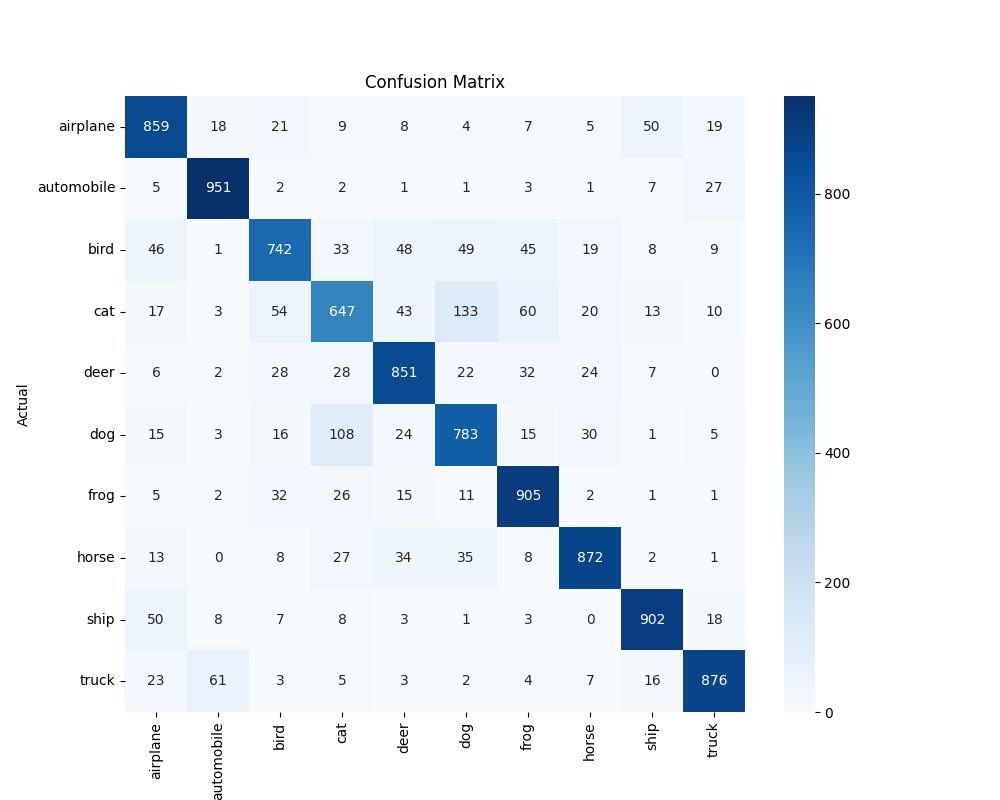
\includegraphics[width=0.7\textwidth]{analysis.png}
\caption{Confusion Matrix}
\label{fig:confusion_matrix}
\end{figure}

\begin{figure}[H]
\centering

\includegraphics[width=0.8\textwidth]{table.png}
\caption{Class Scores}
\label{fig:class_scores}
\end{figure}

\begin{figure}[H]
\centering
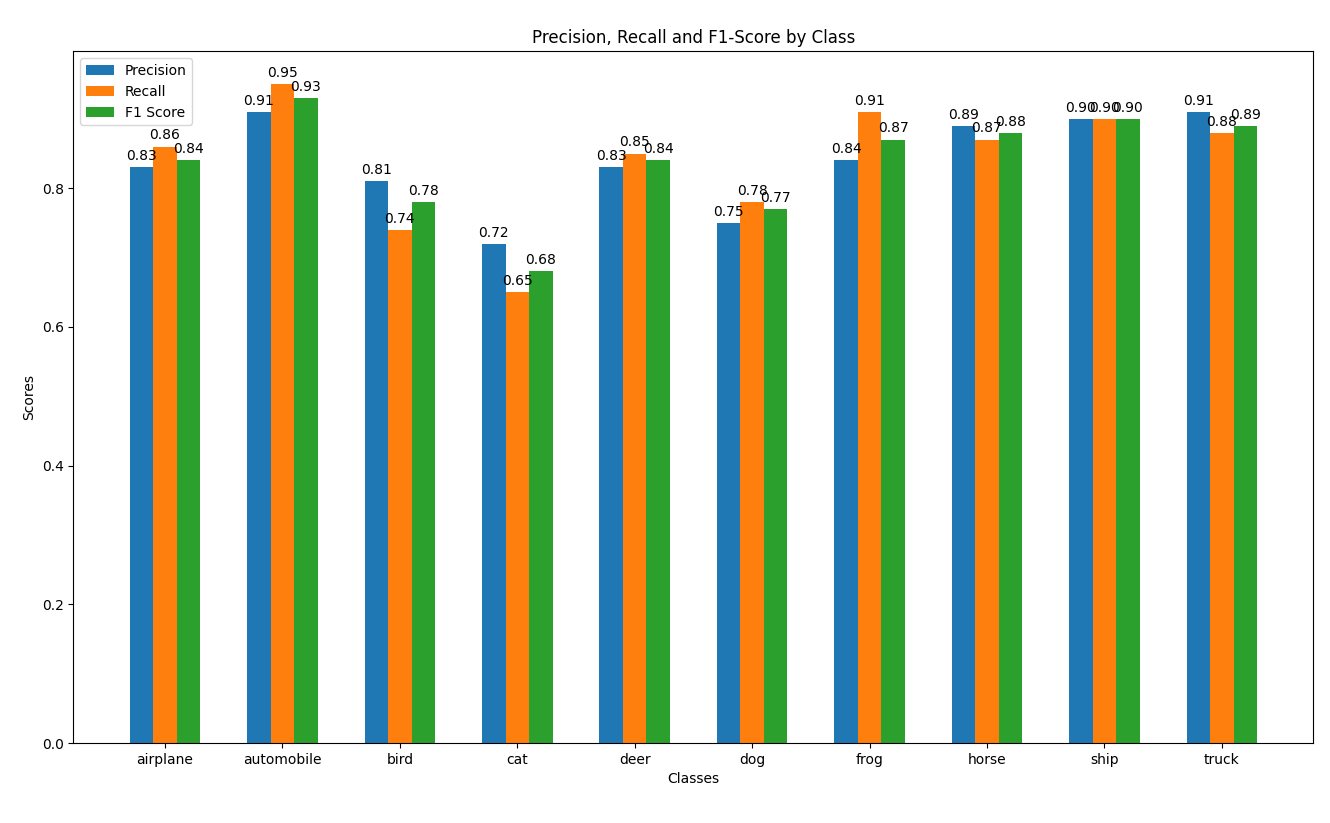
\includegraphics[width=1\textwidth]{scores.png}
\caption{Plot of Class Scores}
\label{fig:scores_plot}
\end{figure}

% \begin{figure}[H]
% \centering
% \includegraphics[width=0.2\textwidth]{Path.png}
% \caption{Final Map with path}
% \label{PMap}
% \end{figure}

\end{document}
